\chapter{Metodología}

En el desarrollo de proyecto, al ser el desarrollo de una aplicación de Software, sumado al corto tiempo asignado para la actividad, se implementará una metodología ágil.

\section{Metodología Ágil}

Día a día, el Software se vuelve más complejo y el manejo de herramientas ha evolucionado, volviéndose más sencillas y productivas de manejar, por ello, se requiere de una metodología de desarrollo de Software que se adapte a estos cambios.
La metodología de desarrollo de Software es un conjunto de "mejores prácticas" que si no se lleva a cabo, resulta inútil\cite{carrizo2018metodo}. Los recursos humanos son considerados como el factor más importante del proyecto de Software.

La metodología ágil de desarrollo de Software se fundamenta en los 4 principios básicos de la figura \ref{manifiesto}, que permite al equipo priorizar el Software que funciona a la documentación, rezagarse del uso de un diagrama relacionales hasta el final del desarrollo y una respuesta a cambios más versátil que en una planificación estricta.
\\
\begin{figure}[t!]
	\centering
	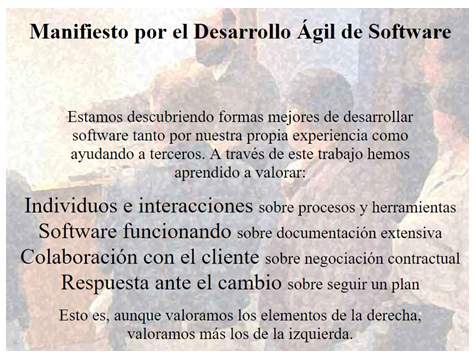
\includegraphics[width=11cm,height=8cm,]{./Images/manifiesto.png}
	\caption{Ejemplo de Clasificación de imagen de TensorFlow}
	\footnotesize Fuente: \cite{beck2001manifiesto}
	\label{manifiesto}
\end{figure}

De las metodologías ágiles conocidas, la más apropiada para el proyecto es la metodología SCRUM, debido a su seguimiento y comunicación, forzando a los miembros a un reporte diario y a un avance continuo con resultados productivos, con la posibilidad de definir metas en un tiempo específico, maximizando la efectividad de los recursos humanos.

\section{Metodología SCRUM}

La metodología SCRUM es una estrategia de gestión donde se aplica un conjunto de prácticas de manera regular para mejorar el trabajo colaborativo y obtener el mejor proyecto de Software posible\cite{scrumdiapo}.

Basado en la adaptabilidad, orientación a las personas y no los procesos y es iterativo e incremental. Requiere de la comunicación directa del cliente con el equipo desarrollador, el cual que será un miembro del equipo, al ser quien expuso, propuso y lideró el desarrollo.

La metodología SCRUM recibe los requisitos y los involucra como parte de la discusión de una reunión, para ser implementada. Se debe garantizar el desarrollo de los requisitos y permite detectar si estos producen conflictos.

\subsection{Componentes de SCRUM}

Para realizar el seguimiento de la metodología SCRUM, se requiere tomar nota de todas las decisiones realizadas, en general, la metodología fue seguida al pie de la letra, sin embargo, se destaca en Plan de Actividades, que hubo una pausa al avance del proyecto durante vasto tiempo, por tanto, se produjeron diversos cortes y extensiones de tiempo al momento de realizar las actividades, posteriormente explicado en dicho subtitulo.

\subsubsection{Roles de la Metodología SCRUM}

\begin{itemize}
	\item \textbf{Product Owner:} Es la persona que conoce el panorama completo del producto y el entorno del negocio, representa a los usuarios del producto y es responsable del seguimiento del proyecto.
	\item \textbf{SCRUM Master:} Encargado de garantizar el funcionamiento de la metodología y evaluar los procesos, es una responsabilidad del funcionamiento del modelo, es un rol flexible del que depende el éxito del proyecto.
	\item \textbf{Project Manager:} Es el encargado de dirigir el equipo a cumplir con los objetivos del equipo, se asegura de que los requerimientos se cumplan.
	\item \textbf{SCRUM Team:} Se le conoce así a los integrantes del equipo de desarrollo, que produce resultados, cuyas habilidades son aptas para el desarrollo del proyecto de Software.
\end{itemize}

Se asigno a cada uno de los integrantes del equipo un rol distintivo y aparte el rol de SCRUM Team.

\subsubsection{Sprint}

Un Sprint es también considerado una iteración y se organiza en la revisión de requisitos del usuario, el cual es la designación de los requisitos del proyecto, traduciéndose tanto en tareas de usuario como en tareas para los desarrolladores,que se distribuyen en los distintos Sprint y deben ser realizadas por el Rol de SCRUM Team. En un Sprint Backlog se realiza el seguimiento de una Sprint, es una pizarra donde se muestran las tareas a realizar en el proyecto, se detallará su funcionamiento.

\subsubsection{Requerimientos}

Los requisitos del usuario, también llamados requerimientos se los considera como un estatuto abstracto en alto nivel de un servicio. Además existen las restricciones del sistema para asegurar una funcionalidad detallada. Los requerimientos tienen las caracterizaras de ser completos, consistentes y precisos. 
La definición de requerimientos tiene que involucrar al cliente, usuario y los roles distintivos (no requiere al SCRUM Team), se debe definir e incluir en un diagrama \ref{futurediagramaderequisitos} los requerimientos para que no existan conflictos entre los interesados y los desarrolladores del proyecto.
La especificación de requerimientos se basa en la formalización y anotación escrita de los requerimientos, normalmente oficializa un contrato entre el cliente y el contratista sobre que se realizará específicamente en el proyecto para evitar demandas y huecos legales, debido a la mala interpretación o subjetividad de los requerimientos solicitados.
Finalmente se realiza la especificación del Software, que es una descripción más detallada del Software, que servirá como base para el diseño e implementación de los requerimientos, esta es manejada por el SCRUM Team.

\subsubsection{Tareas y Estimación de Poker}

Los requerimientos se transforman en tareas, básicamente es reescrito para ser entendido y manejado por el SCRUM Team que realizaran las tareas, para realizar un seguimiento del tiempo que el equipo trabaja y se toma en realizar cada tarea, se debe reunir al SCRUM Team e indagar cuanto tiempo se estimará a cada tarea, para este proyecto, se empleo el método Estimación de Poker.

Estimación de Poker es una técnica de un riesgo elevado en metodologías Ágiles, es una herramienta de asignación de tiempo requerido para realizar una tarea, que reúne a todo el SCRUM Team para realizar una estimación individual sobre la cantidad de tiempo que llevaría realizar esa actividad a través de cartas y una escala de tiempo, en este caso, de horas de 1 a 13 horas, para determinar los motivos que tiene esa persona para dar ese tiempo y llegar a un consenso sobre el tiempo requerido \cite{scrumdiapo}. Este método de estimación se empleo también para definir el tiempo de trabajo diario en que se trabajaría el proyecto.

Posteriormente, durante el proceso de elaboración de cada tarea asignada, se descubrió una realidad totalmente distinta a los números estimados, siendo indefinidamente mayores a los estimados, por tanto se tuvo que trabajar al menos 3 veces más el estimado para la mayoría de las tareas, detallado en el Product Backlog.

\subsubsection{Reuniones}

Las reuniones deben ser diarias y por Sprint, las cuales tienen el objetivo de definir cual es el trabajo que se debe realizar durante el Sprint. Para una reunión con la metodología SCRUM, deben participar todos los roles para poder generar la lista de tareas a realizar, además de determinar el objetivo de la Sprint.

Durante el transcurso del proyecto, en las reuniones diarias realizadas a horas \textbf{09:45-10:00}, se debe reportar 3 puntos del avance de los integrantes del SCRUM Team, que son el trabajo realizado, el trabajo a realizar y los problemas encontrados. Este punto de la metodología fue realizado con éxito.

\subsubsection{Sprint Backlog}

El Sprint Backlog es una pizarra donde se muestran las tareas a realizar en el proyecto, para el proyecto, se definió el uso de la herramienta \href{https://hacknplan.com/}{HacknPlan}, que es una pagina web dedicada a la administración de proyectos, brinda un servicio excepcional para la creación de un Sprint Backlog de la metodología ágil SCRUM, la cual fue recomendada por el Docente de Ingeniería de Software.
\\
La Sprint Backlog tiene 4 secciones descritas en la tabla \ref{sprintbacklog} y visualmente representadas en la figura \ref{sprintexample} que se encuentra en la sección de anexos.


\begin{table}[t]
	\begin{center}
		\begin{tabular}{| m{3cm} | m{11cm} |  }
			\hline Planificado & Las tareas traducidas para la facilidad del SCRUM Team y su resolución. \\ \hline
			En Progreso & Tareas que actualmente están siendo elaboradas por al menos un miembro del SCRUM Team. \\ \hline
			Pruebas & Tareas que han sido terminadas, pero requieren de una búsqueda de errores o aprobación del SCRUM Master. \\ \hline
			Completado & Son las tareas finalizadas, aquellas que ya no requieren cambios y han sido aprobadas por el SCRUM Master y confirmadas por el Project Manager.  \\ \hline
		\end{tabular}
		\caption{Secciones de un Sprint Backlog}
		\label{sprintbacklog}
		\footnotesize Fuente: Elaboración Propia basado en la Herramienta HacknPlan.
	\end{center}
\end{table}

Las tareas requieren de un formato para poder ser manejadas por el SCRUM Team y supervisadas por los demás roles, las secciones que componen una tarea son descritas en la tabla \ref{sprinttabla}. En la figura \ref{sprinttarea} de la sección de anexos, se puede observar un ejemplo de una tarea completada.

\begin{table}[t]
	\begin{center}
		\begin{tabular}{| m{4cm} | m{10cm} |  }
			\hline Titulo & El alias de la historia (tarea), se le asigna un nombre corto. \\ \hline
			 Importancia & Se determina su importancia en 3 niveles, bajo, normal o alta. \\ \hline
			 Estimación Inicial & Se determina el tiempo que toma la actividad, previamente definido con Planning Poker \\ \hline
			 Descripción & Lo que se busca realmente, el requerimiento funcional que se necesita para la elaboración de la tarea, se detalla lo que se requiere, esta sección es empleada solo para las tareas de programación. \\ \hline
			 Comentarios & Se describen los avances, problemas encontrados y varios a medida que se desarrolla o termina la tarea. \\ \hline
			Registro de trabajo  & Acompañado de un comentario donde se registra que se hizo, se anota cuanto tiempo estuvieron que miembros del SCRUM Team en la tarea. \\ \hline
		\end{tabular}
		\caption{Secciones de una tarea dentro del Sprint Backlog}
		\label{sprinttabla}
		\footnotesize Fuente: Elaboración Propia basado en la Herramienta HacknPlan.
	\end{center}
\end{table}

\subsubsection{Product Backlog}

El Product Backlog es una lista de requisitos o tareas que representa la visión y expectativa del cliente respecto a objetivos y entregas del proyecto. Se debe mencionar el valor y el costo de su finalización. Se puede observar el Product Backlog en la tabla \ref{productbacklog}.

En la tabla, se observan los campos:
\begin{itemize}
	\item ID como identificador de la tarea, debe ser único.
	\item Tarea, que indica el título dado en Sprint Backlog para facilitar su comprensión.
	\item Estado(Sprint), si ha de estar Planificada, En Proceso o Hecho (Sprint en que se realizo) o si fue Descartado.
	\item Valor, el valor designado a cada actividad realizada, en total se asignan 1000 puntos a su finalización
	\item Estimado Inicial, la valoración de las tareas que se mide en horas requeridas.
	\item Factor Ajuste, determina el fallo que se debe aumentar al tiempo original, se le suma al Valor Estimado en función $Valor Estimado = Valor Estimado + Valor Estimado * Factor de Ajuste$
	\item Ajustado, es la valoración de las tareas posteriormente al ser más realistas sobre el tiempo requerido para resolverlo.
	\item Sprint, que señala el número de Sprint en que fue realizada
	\item  Prioridad, al ser una metodología ágil, se reconoce que las tareas pueden ser más relevantes unas que otras, en este caso, Baja, Normal y Alta.

\end{itemize}
La Tarea es el nombre dado a las tareas distribuidas al SCRUM Team, formuladas a partir de los requerimientos del cliente.
El valor de las tareas se distribuirá de un valor total de 1000 puntos, se determinara una cuarta parte a la redacción del informe, una cuarta parte a la investigación dedicada requerido para poder hacer posible el proyecto y el resto lo determinará el rol de Product Owner.
El Estimado Inicial es definido con la Estimación de Poker previamente mencionada.
Redactar en la tabla \ref{productbacklog} engloba la redacción del informe y el tiempo estimado de cada tarea de redacción, el Redactar hace referencia a los títulos de cada parte del informe.
En Redactar Parte 1, están los títulos de Objetivos, Estudio de Diagnóstico, Marco Teórico, Estudio de Alternativas, Plan de Actividades
En Redactar Parte 2, están los títulos de Metodología, Diseño, Conclusiones, Recomendaciones, dentro de la metodología se lleva a cabo la tarea de Seguimiento de Product Owner.
En Redactar Parte 3, están los títulos de Introducción, Anexos, Glosario, Revisión de ortografía y Resumen.
\restoregeometry
\newgeometry{left=0.5cm,bottom=.25cm}
\begin{landscape}
\begin{table}[t]
	\begin{center}
		\begin{tabular}{| c | c | c | c | c | c | c | c | c |}
			\hline
			\multicolumn{9}{ |c| }{Product Backlog} \\ \hline
			ID & Tarea & Estado(Sprint) & Valor & Estimado Inicial (h)& Factor Ajuste & Ajustado(h) & Sprint & Prioridad \\ \hline
			T-0 & Redactar Parte 1 & Hecho(1) & 50 & 18 & 1.5 & 40 & 1 & Normal \\ \hline
			T-1 & Redactar Parte 2 & (2) & 100 & 20 &  &  & 2 & Normal \\ \hline
			T-1 & Redactar Parte 3 & (3) & 100 & 9 &  &  & 3 & Normal \\ \hline
			T-2 & Investigación de Herramientas & Hecho(1) & 250 & 24 & 3.0 & 96 &  1 & Normal \\ \hline
			T-3 & Manipulación de Herramientas & Hecho(1) &  & 12 & 1.0 & 24 & 1 & Normal \\ \hline
			T-4 & Modificación de GUI & Hecho(1) &  &  & &  & 1 & Baja \\ \hline
			T-5 & Mostrar Video a Copiar en la Pantalla & Hecho(1) &  &  & &  & 1 & Alta \\ \hline
			T-6 & Lectura de Movimientos del Usuario & Hecho(1) &  &  & &  & 1 & Alta \\ \hline
			T-7 & Redimension de Imagen para Comparar & Hecho(1) &  &  & &  & 1 & Alta \\ \hline
			T-8 & Menú y Boton Play de Redireccionamiento & Hecho() &  &  & &  &  & Normal \\ \hline
			T-9 & Calificación de Movimientos & Hecho(2) &  & 10 &  &  & 2 & Alta \\ \hline
			T-10 & Mostrar acciones a copiar & Hecho() &  & 3 & &  &  & Alta \\ \hline
			T-15 &  & Hecho() &  &  & &  &  & Normal \\ \hline
			 & Entrega final & & 1000 &  &  & 900 &  &  \\ \hline
		\end{tabular}
		\caption{Product Backlog}
		\label{productbacklog}
		\footnotesize Fuente: Elaboración propia
	\end{center}
\end{table}
\end{landscape}
\restoregeometry

\subsubsection{Gráfica Burn-Up}

Es una herramienta de seguimiento que se usa en la metodología ágil SCRUM, sirve para determinar el tiempo estimado del proyecto en general, para tener una referencia visual de cuanto progreso se realizo realmente, se establecieron los siguientes puntos:

\begin{itemize}
	\item Versión 0.1: Tiempo en que se estima tendrá una demo para presentar.
	\item Horas Estimadas de Trabajo: Cantidad de horas totales estimadas para la realización del proyecto.
	\item Horas Acumuladas: Cantidad de horas registradas durante los Sprint para cada tarea que tiene progreso, no necesariamente terminadas para sumarlas a la gráfica. 
	\item Trayectoria Estimada: La estimación optimista de la distribución de horas, determina la trayectoria de las horas acumuladas deseada.
\end{itemize}

Para estimar la cantidad de horas de trabajo se empleará un calculo simple.
 Primero se estiman 3 horas en promedio en un rango de 2 a 5 horas de trabajo diario mientras la Sprint este activa, se toma en cuenta que se trabajaran todos los. La estimación de tiempo toma en cuenta que la fecha de inicio del proyecto es el 17 de Septiembre y la fecha de entrega estimada es el 14 a 17 de Diciembre, determinando un total de 88 días mínimo, se las multiplica y redondea al dígito más grande como se ve en la ecuación \ref{eqn:horasestimadas}.
 
\begin{equation} 
\label{eqn:horasestimadas} 
	792 \text{ Horas Estimadas de Trabajo} = 3 \text{ Horas Diarias} * 3 \text{ Personas} * 88 \text{ Días disponibles}	
\end{equation}

La cantidad de horas estimadas se redondea a 800 horas, este es un calculo pesimista, tomando en cuenta que el desconocimiento inicial de las herramientas con las que se trabajan y el tiempo que tome resolver problemas sea muy elevado, que durante el desarrollo se demuestra que es necesario.

\subsubsection{Gráfica Burn-Down}

Es una herramienta de seguimiento que se usa en la metodología ágil SCRUM, sirve para determinar el tiempo estimado que se tiene en total para cada tarea y todas las tareas, para tener una referencia visual de cuanto progreso se ha completado en comparación al ideal, se establecieron los siguientes puntos:

\begin{itemize}
	\item Remanente Ideal: En una trayectoria descendiente deseada para estimar resultados, se observa la cantidad de horas que faltan para  llegar a la meta.
	\item Esfuerzo Remanente: Es la cantidad de horas que todavía faltan por registrar por parte del SCRUM Team.
	\item Tareas Remanentes: Cantidad de tareas totales de las Sprint que faltan por completar.
	\item Tareas Completadas: Tareas realizadas durante ese espacio de tiempo especifico. 
\end{itemize}
				




